% =============================================================================
% Module 4: The Gravitational Lens Equation
% =============================================================================
% Sources: Narayan & Bartelmann Sec. 2.1.3-2.1.5, Congdon & Keeton Ch. 2 & 4,
%          Saha et al. Sec. 1
% Mathematica: ../Mathematica/04_Lens_Equation/
% =============================================================================

\chapter{The Gravitational Lens Equation}
\label{ch:lens_equation}

\begin{quote}
\textit{Equation (14) is called the lens equation, or ray-tracing equation.  It is
nonlinear in the general case, and so it is possible to have multiple images
$\vec\theta$ corresponding to a single source position $\vec\beta$.}
\hfill --- Narayan \& Bartelmann (1997), Sect.~2.1.3
\end{quote}

\noindent
In Module~\ref{ch:light_deflection} we derived the deflection angle
$\alphahat = 4\Gnewton M / (\speedoflight^2 b)$ for a point mass, and
in Module~\ref{ch:linearized_gravity} we showed that deflection angles
from multiple masses superpose in the weak-field limit.  In
Module~\ref{ch:cosmological_distances} we introduced the angular diameter
distances $\Dd$, $\Ds$, and $\Dds$ that describe the geometry of the
observer--lens--source system at cosmological separations.

Now we assemble these ingredients into the \textbf{lens equation} ---
the fundamental mapping from source positions to image positions.  This
single equation is the starting point for everything that follows:
image multiplicity, magnification, time delays, and lens modeling.

\medskip
\noindent
\textbf{Companion Mathematica files:}
\begin{itemize}[nosep]
    \item \mathlink{04_Lens_Equation/lens_equation.wl}{lens\_equation.wl}
          --- symbolic derivation of the lens equation, Einstein radius,
          point mass image positions, magnification preview, critical
          surface mass density, and publication-quality figure generation
    \item \mathlink{04_Lens_Equation/einstein_ring.nb}{einstein\_ring.nb}
          --- interactive notebook: Manipulate for source position and
          image positions, Einstein ring visualization, interactive
          $\thetaE$ calculator
\end{itemize}


% =====================================================================
\section{Introduction: From Deflection to Imaging}
\label{sec:lens_eq_intro}

We now have all the pieces needed to build the gravitational lens
equation:
\begin{enumerate}
    \item \textbf{The deflection angle} (Modules~1e and~2):
          $\alphahat = 4\Gnewton M / (\speedoflight^2 b)$ for a point
          mass, and the superposition
          principle~\eqref{eq:superposition_deflection} for multiple
          masses and continuous distributions.
    \item \textbf{The cosmological distances} (Module~3): the angular
          diameter distances $\Dd$, $\Ds$, $\Dds$ relating angular
          separations on the sky to physical separations at the lens
          and source.
\end{enumerate}
The task of this module is to combine these into a single equation
that maps source positions $\vecbeta$ to image positions $\vectheta$.
Remarkably, this equation can produce \textit{multiple solutions} ---
multiple images of a single source --- which is the defining
phenomenon of strong gravitational lensing.


% =====================================================================
\section{The Thin-Screen Approximation}
\label{sec:thin_screen}

The physical extent of a gravitational lens along the line of sight is
typically much smaller than the distances between observer, lens, and
source.  For a galaxy lens, the stellar and dark matter distribution
extends over $\sim 100$~kpc, while $\Dd \sim 1$~Gpc.  For a galaxy
cluster, the virial radius is $\sim 2$~Mpc, compared to distances of
several Gpc.  In both cases the ratio
\begin{equation}
    \frac{\text{lens extent}}{\text{cosmological distance}}
    \sim \frac{100~\text{kpc}}{1~\text{Gpc}} = 10^{-4}
    \label{eq:thin_screen_ratio}
\end{equation}
is exceedingly small.

\begin{remark}
The thin-screen approximation is the gravitational analog of the
\textbf{thin-lens} approximation in classical optics.  Just as a glass
lens can be treated as imparting a phase shift at a single plane
(when its thickness is much less than the focal length), a
gravitational lens can be treated as deflecting light at a single
\textbf{lens plane} perpendicular to the line of sight at distance
$\Dd$.
\end{remark}

This justifies the following idealization: all the mass of the lens is
projected onto a single plane (the \textbf{lens plane}) at angular
diameter distance $\Dd$ from the observer.  The deflection of a light
ray occurs instantaneously as it crosses this plane.  The three-dimensional
mass distribution $\rho(\mathbf{r})$ is replaced by a two-dimensional
\textbf{surface mass density} $\Sigma(\vecxi)$, obtained by integrating
$\rho$ along the line of sight:
\begin{equation}
    \Sigma(\vecxi) = \int_{-\infty}^{+\infty} \rho(\vecxi, z)\, dz \,,
    \label{eq:surface_mass_density_def}
\end{equation}
where $\vecxi$ is the two-dimensional position in the lens plane and $z$
is the coordinate along the line of sight.
\begin{annotation}[What the thin screen throws away]
Two things are discarded, and it is worth knowing which. (i) \emph{Where along
the line of sight} the deflection happens: a ray crossing a galaxy is bent
gradually over $|z| \lesssim 100$~kpc, but because that path is
$\sim 10^{-4}$ of $\Dd$ (eq.~\ref{eq:thin_screen_ratio}), replacing the gradual
bend by one kink at $z = 0$ changes positions at the same relative level.
(ii) \emph{How the mass is distributed along $z$}: only the projection
$\Sigma(\vecxi)$ survives. Two lenses with very different $\rho(\vecxi, z)$ but
the same $\Sigma$ are indistinguishable to lensing. That is why lensing
measures projected masses, and it is why extra information such as
stellar kinematics is needed to see the third dimension
(Module~\ref{ch:galaxy_lensing}).

The thin-screen idealization applies to \emph{each} deflector separately. When two
deflectors sit at very different distances (a lens galaxy and a second
galaxy behind it), one screen is not enough and each gets its own plane. That is
the multi-plane problem of Part~V.
\end{annotation}


% =====================================================================
\section{Lensing Geometry}
\label{sec:lensing_geometry}

Figure~\ref{fig:lensing_geometry} shows the geometry of a typical
gravitational lensing configuration.  The key elements are:

\begin{itemize}
    \item \textbf{Observer (O):} located at the bottom of the diagram.
    \item \textbf{Lens plane:} a plane perpendicular to the optical
          axis at angular diameter distance $\Dd$ from the observer.
          The lens (galaxy, cluster, etc.) is projected onto this plane.
    \item \textbf{Source plane:} a plane perpendicular to the optical
          axis at angular diameter distance $\Ds$ from the observer.
          The background source (galaxy, quasar, etc.) lies in this
          plane.
    \item \textbf{Optical axis:} the line from the observer through
          the center of the lens, defining the origin of the angular
          coordinate system.
\end{itemize}

We define the following angles (all measured from the optical axis):
\begin{itemize}
    \item $\vectheta$: the \textbf{observed image position} on the sky,
    \item $\vecbeta$: the \textbf{true source position} (where the source
          would appear without lensing),
    \item $\alphahat$: the \textbf{physical deflection angle} at the
          lens plane,
    \item $\vecalpha(\vectheta)$: the \textbf{reduced deflection angle},
          defined below.
\end{itemize}

The physical positions in the lens and source planes are related to the
angular positions by:
\begin{align}
    \vecxi &= \Dd\, \vectheta \,, \label{eq:xi_theta} \\
    \veceta &= \Ds\, \vecbeta \,, \label{eq:eta_beta}
\end{align}
where $\vecxi$ is the position in the lens plane and $\veceta$ is the
position in the source plane
(Narayan \& Bartelmann eq.~15; Congdon \& Keeton Sec.~2.2.2).
\begin{annotation}[Angular-diameter distances, and why $\Dds \neq \Ds - \Dd$]
Equations~\eqref{eq:xi_theta}--\eqref{eq:eta_beta} are not approximations to
be justified; they are the \emph{definition} of angular-diameter distance,
``separation $=$ angle $\times$ distance'' (Narayan \& Bartelmann eq.~15).
The lens-to-source distance $\Dds$ is defined the same way, but for an
observer sitting at the lens. Because space expands while the light travels,
these distances do not add. For the fiducial lens of this chapter
($z_d = 0.3$, $z_s = 1$, flat $\Lambda$CDM with $\Omegam = 0.3$):
$\Ds - \Dd = 1652 - 919 = 733$~Mpc, while $\Dds = 1055$~Mpc. In a flat
universe the correct combination is
$(1+z_s)\,\Dds = (1+z_s)\,\Ds - (1+z_d)\,\Dd$
(differences of comoving distances, Module~\ref{ch:cosmological_distances}).

\emph{Classic error:} computing $\Dds$ as $\Ds - \Dd$. Here it would
underestimate $\Dds/\Ds$, and hence every deflection, by about 30\%.
\end{annotation}

\begin{figure}[ht]
    \centering
    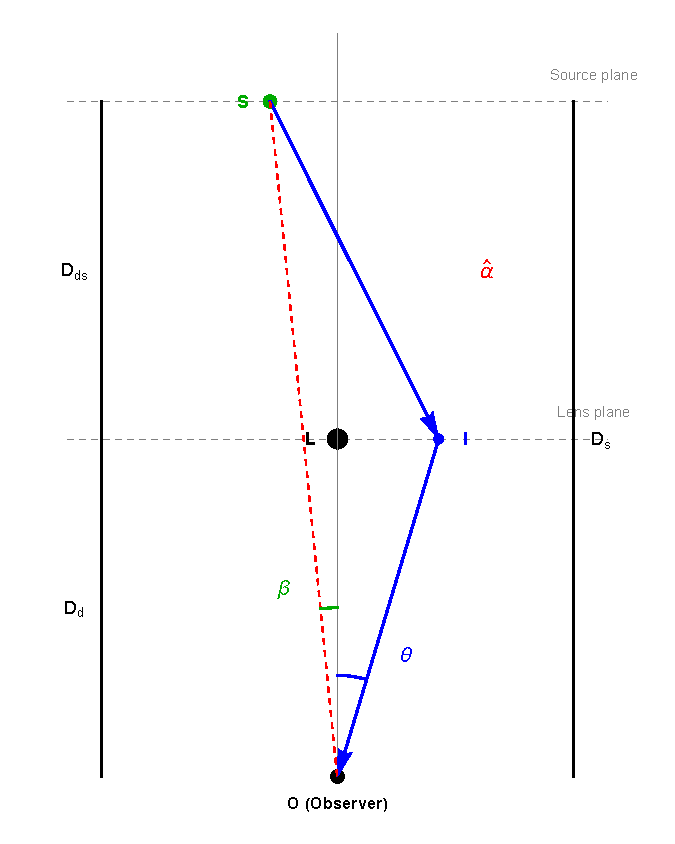
\includegraphics[width=0.78\textwidth]{../Figures/04_Lens_Equation/lensing_geometry.pdf}
    \caption{Geometry of gravitational lensing.  A light ray from a
    source at angular position $\vecbeta$ in the source plane is
    deflected by the angle $\alphahat$ as it passes through the lens
    plane, and is observed at angular position $\vectheta$.  The
    angular diameter distances $\Dd$, $\Ds$, and $\Dds$ connect
    angular separations to physical separations.  The reduced
    deflection angle $\vecalpha = (\Dds/\Ds)\,\boldsymbol{\hat{\alpha}}$
    gives the apparent angular shift.  Generated by
    \texttt{lens\_equation.wl}.}
    \label{fig:lensing_geometry}
\end{figure}


% =====================================================================
\section{The Lens Equation}
\label{sec:lens_equation}

From the geometry of Figure~\ref{fig:lensing_geometry}, we can read off
the fundamental relationship between source and image positions.  A light
ray that is observed at angle $\vectheta$ from the optical axis was
emitted from the source at position $\veceta$ in the source plane.
Following the deflected ray from the lens plane to the source plane, the
physical displacement in the source plane is
(Narayan \& Bartelmann Sec.~2.1.3; Congdon \& Keeton eq.~2.16):
\begin{equation}
    \veceta = \frac{\Ds}{\Dd}\, \vecxi
    - \Dds\, \boldsymbol{\hat{\alpha}}(\vecxi) \,.
    \label{eq:eta_physical}
\end{equation}
Substituting $\vecxi = \Dd\,\vectheta$ and
$\veceta = \Ds\,\vecbeta$:
\begin{equation}
    \Ds\, \vecbeta = \Ds\, \vectheta
    - \Dds\, \boldsymbol{\hat{\alpha}}(\Dd\,\vectheta) \,,
\end{equation}
and dividing by $\Ds$:
\begin{equation}
    \boxed{
    \vecbeta = \vectheta
    - \frac{\Dds}{\Ds}\, \boldsymbol{\hat{\alpha}}(\Dd\,\vectheta)
    }
    \label{eq:lens_equation_full}
\end{equation}
\begin{derivation}[Reading eq.~\eqref{eq:eta_physical} off the geometry]
Follow the ray \emph{backwards} from the observer, who sees it arrive from
direction $\vectheta$.
\begin{enumerate}
    \item \emph{Observer to lens plane.} The ray travels in a straight line and
          meets the lens plane at transverse position $\vecxi = \Dd\vectheta$
          (definition of $\Dd$).
    \item \emph{If there were no lens,} the same straight line would reach the
          source plane at $\Ds\vectheta = (\Ds/\Dd)\,\vecxi$ (definition of $\Ds$).
    \item \emph{The kink.} At the lens plane the ray was bent by
          $|\alphahat|$ toward the mass. With the sign convention of
          eq.~\eqref{eq:deflection_integral_continuous}, the vector
          $\boldsymbol{\hat{\alpha}}$ points from the mass toward the ray
          (along $\vecxi - \vecxi'$). The true ray therefore leaves the lens
          plane tilted by $-\boldsymbol{\hat{\alpha}}$ relative to the straight
          continuation.
    \item \emph{Lens plane to source plane.} Two lines leaving the same point
          with angular separation $|\alphahat|$ are $\Dds|\alphahat|$ apart at
          the source plane (definition of $\Dds$). Hence
          $\veceta = (\Ds/\Dd)\vecxi - \Dds\boldsymbol{\hat{\alpha}}$, which is
          eq.~\eqref{eq:eta_physical}.
\end{enumerate}
The exact flat-geometry relation is
$\Ds\tan\beta = \Ds\tan\theta - \Dds\tan\alphahat$ (Congdon \& Keeton
eq.~2.15). Since $\tan x / x = 1 + x^2/3 + \mathcal{O}(x^4)$, the
small-angle replacement $\tan x \to x$ is wrong only at relative order
$x^2/3$: below $2\times10^{-8}$ even for a $37''$ cluster Einstein radius.
Dividing by $\Ds$ then gives eq.~\eqref{eq:lens_equation_full} with no
further approximation.
\end{derivation}

This is the \textbf{gravitational lens equation} in terms of the physical
deflection angle $\boldsymbol{\hat{\alpha}}$.  It is convenient to define
the \textbf{reduced deflection angle}:
\begin{equation}
    \boxed{
    \vecalpha(\vectheta) \equiv \frac{\Dds}{\Ds}\,
    \boldsymbol{\hat{\alpha}}(\Dd\,\vectheta)
    }
    \label{eq:reduced_deflection}
\end{equation}
so that the lens equation takes the elegant form:
\begin{equation}
    \boxed{
    \vecbeta = \vectheta - \vecalpha(\vectheta)
    }
    \label{eq:lens_equation}
\end{equation}
\begin{annotation}[Physical vs.\ reduced deflection]
$\alphahat$ is the actual bend of the ray at the lens. It depends only on the
mass and the \emph{physical} impact parameter $\xi$, and it knows nothing
about where the source is. $\vecalpha$ is the \emph{apparent} angular shift
seen from Earth, a fraction $\Dds/\Ds$ of the bend: a kink close to the
source (small $\Dds/\Ds$) hardly moves the image. For the fiducial lens
($z_d = 0.3$) this ``lensing efficiency'' is $\Dds/\Ds = 0.64$ for $z_s = 1$
and $0.77$ for $z_s = 2$. The same galaxy deflects the more distant source
through a larger apparent angle.

\emph{Classic errors:} (i) inserting $\alphahat = 4\Gnewton M/(\speedoflight^2 b)$
directly into $\vecbeta = \vectheta - \vecalpha$ without the factor $\Dds/\Ds$;
(ii) evaluating $\alphahat$ at the angle $\theta$ instead of the physical
radius $\xi = \Dd\theta$. Both $\alpha$ and $\alphahat$ are in radians,
while $\xi$ carries units of length.
\end{annotation}
\begin{bridge}[Multi-plane lensing]
Chapter~\ref{ch:multiplane_dspl} applies eq.~\eqref{eq:lens_equation_full}
once per plane. A deflector on plane $j$ contributes to the position of a ray on a
later plane $k$ with weight $D_{jk}/D_k$. This is exactly the efficiency factor
$\Dds/\Ds$ of this section with $(d, s) \to (j, k)$
(Schneider, Ehlers \& Falco Sec.~9.1). For a double-source-plane lens, the ratio of the
two efficiencies behind a common deflector,
$\Brat = (D_{ds_1}/D_{s_1})/(D_{ds_2}/D_{s_2})$, is the cosmology-sensitive
observable. For $z_d = 0.3$, $z_{s_1} = 1$, $z_{s_2} = 2$ it is
$\Brat = 0.83$.
\end{bridge}

\begin{remark}
Equation~\eqref{eq:lens_equation} is \textbf{THE} fundamental equation
of gravitational lensing.  Every result in strong lensing theory ---
image positions, magnifications, time delays, critical curves, caustics
--- derives from this single equation.  The nonlinearity of the
deflection angle $\vecalpha(\vectheta)$ is what allows multiple
solutions (multiple images) for a given source position $\vecbeta$.
\end{remark}

\begin{remark}
The lens equation is a mapping from the image plane to the source plane:
given an image position $\vectheta$, it determines the corresponding
source position $\vecbeta$.  The \textit{inverse} problem --- given a
source position $\vecbeta$, find all image positions $\vectheta$ --- is
generally much harder, because the equation can have multiple solutions.
For a point mass lens the inverse problem can be solved analytically
(Section~\ref{sec:einstein_radius}); for more complex lens models it
typically requires numerical root-finding.
\end{remark}


% =====================================================================
\section{Surface Mass Density and the Deflection Integral}
\label{sec:surface_mass_density}

For a continuous mass distribution described by the surface mass density
$\Sigma(\vecxi)$ (eq.~\ref{eq:surface_mass_density_def}), the physical
deflection angle at position $\vecxi$ in the lens plane is obtained by
superposing the deflections from all mass elements
(Congdon \& Keeton eq.~4.9; cf.\ Module~1e
eq.~\ref{eq:continuous_deflection}):
\begin{equation}
    \boxed{
    \boldsymbol{\hat{\alpha}}(\vecxi) = \frac{4\Gnewton}{\speedoflight^2}
    \int \frac{(\vecxi - \vecxi')\, \Sigma(\vecxi')}
    {|\vecxi - \vecxi'|^2}\, d^2\xi'
    }
    \label{eq:deflection_integral_continuous}
\end{equation}

This is the two-dimensional analog of the Newtonian gravitational field
of a surface mass distribution.  The integral extends over the entire
lens plane.  In terms of the angular position $\vectheta$ and using
$\vecxi = \Dd\,\vectheta$, the reduced deflection angle becomes:
\begin{equation}
    \vecalpha(\vectheta) = \frac{\Dds}{\Ds}\,
    \frac{4\Gnewton}{\speedoflight^2}\, \Dd
    \int \frac{(\vectheta - \vectheta')\, \Sigma(\Dd\,\vectheta')}
    {|\vectheta - \vectheta'|^2}\, d^2\theta' \,.
    \label{eq:alpha_angular}
\end{equation}
\begin{derivation}[From $\vecxi$ to $\vectheta$ in the deflection integral]
Substitute $\vecxi = \Dd\vectheta$ and $\vecxi' = \Dd\vectheta'$ in
eq.~\eqref{eq:deflection_integral_continuous}, term by term:
\begin{itemize}
    \item numerator: $\vecxi - \vecxi' = \Dd(\vectheta - \vectheta')$;
    \item denominator: $|\vecxi - \vecxi'|^2 = \Dd^2|\vectheta - \vectheta'|^2$;
    \item area element: $d^2\xi' = \Dd^2\, d^2\theta'$ (each of the two
          coordinates scales by $\Dd$).
\end{itemize}
The powers of $\Dd$ combine as $\Dd \cdot \Dd^2 / \Dd^2 = \Dd$, so
$\alphahat = (4\Gnewton\Dd/\speedoflight^2)\int(\vectheta - \vectheta')
\Sigma(\Dd\vectheta')\,|\vectheta - \vectheta'|^{-2}\,d^2\theta'$. Multiplying by
$\Dds/\Ds$ gives eq.~\eqref{eq:alpha_angular}. The prefactor is
\begin{equation*}
    \frac{\Dds}{\Ds}\,\frac{4\Gnewton}{\speedoflight^2}\,\Dd
    = \frac{1}{\pi}\,\frac{4\pi\Gnewton}{\speedoflight^2}\,\frac{\Dd\Dds}{\Ds}
    = \frac{1}{\pi\,\Sigmacr}
\end{equation*}
with $\Sigmacr$ from eq.~\eqref{eq:sigma_cr} below. So
$\vecalpha(\vectheta) = \frac{1}{\pi}\int\kappab(\vectheta')
(\vectheta - \vectheta')\,|\vectheta - \vectheta'|^{-2}\,d^2\theta'$, the
form used throughout Module~\ref{ch:magnification}. All distance factors have
disappeared into $\kappab$.
\end{derivation}

\begin{remark}
The deflection integral~\eqref{eq:deflection_integral_continuous} follows directly
from the superposition principle derived in Module~\ref{ch:linearized_gravity}
(eq.~\ref{eq:superposition_deflection}).  Each infinitesimal mass element
$\Sigma(\vecxi')\, d^2\xi'$ acts as a point mass, deflecting the light
ray by $4\Gnewton \Sigma(\vecxi')\,d^2\xi' / (\speedoflight^2\, |\vecxi -
\vecxi'|)$ in the direction of $(\vecxi - \vecxi') / |\vecxi - \vecxi'|$.
Superposition (valid because we are in the weak-field regime) gives the
total deflection as the integral over the lens plane.
\end{remark}
\begin{annotation}[The two-dimensional shell theorem]
For a circularly symmetric $\Sigma$ the integral collapses. Put the ray at
$(\xi, 0)$ and a ring of mass at radius $r$. The angular integral of the
$x$-component of the kernel is
$\int_0^{2\pi}(\xi - r\cos\phi)/(\xi^2 + r^2 - 2\xi r\cos\phi)\,d\phi = 2\pi/\xi$
for $r < \xi$ and $0$ for $r > \xi$. Rings outside the ray exert no net pull,
and rings inside act as if their mass sat at the centre. Hence
$\alphahat(\xi) = 4\Gnewton M(<\xi)/(\speedoflight^2\xi)$, where $M(<\xi)$ is the
projected mass inside $\xi$. The next section uses this result for the uniform
disk.
\end{annotation}


% =====================================================================
\section{Critical Surface Mass Density}
\label{sec:critical_density}

There is a natural surface mass density at which the lens is just
strong enough to bend a ray from the source back to the optical
axis.  Consider a uniform disk of constant surface mass density
$\Sigma$, and ask what $\Sigma$ is required for the disk to act as
a perfect focusing lens for a source at infinity, i.e., $\alpha(\theta)
= \theta$ for every $\theta$ inside the disk.

For a uniform disk the two-dimensional enclosed mass within
$\xi = \Dd\theta$ is $M_{\mathrm{2D}}(\xi) = \pi\xi^2\Sigma$, so
the physical deflection
$\alphahat = 4\Gnewton M_{\mathrm{2D}}/(\speedoflight^2\xi)
= 4\pi\Gnewton\Sigma\,\xi/\speedoflight^2$.
Converting to the reduced deflection via
$\vecalpha = (\Dds/\Ds)\,\alphahat$ and $\xi = \Dd\theta$:
\begin{equation*}
    \alpha(\theta) \;=\; \frac{\Dds}{\Ds}\cdot
        \frac{4\pi\Gnewton\Sigma\,\Dd\,\theta}{\speedoflight^2}.
\end{equation*}
The focusing condition $\alpha(\theta) = \theta$ removes the factor
of $\theta$ and gives $\Sigma = \Sigmacr$ with
(Narayan \& Bartelmann eq.~17; Congdon \& Keeton eq.~2.68):
\begin{equation}
    \boxed{
    \Sigmacr = \frac{\speedoflight^2}{4\pi \Gnewton}
    \,\frac{\Ds}{\Dd\, \Dds} \,.}
    \label{eq:sigma_cr}
\end{equation}
\begin{derivation}[The focusing condition, line by line]
By the shell theorem (previous annotation), a uniform disk deflects a ray at
$\xi$ as if the enclosed mass $M_{\mathrm{2D}} = \pi\xi^2\Sigma$ sat at the
centre:
\begin{align*}
    \alpha(\theta)
    &= \frac{\Dds}{\Ds}\,\frac{4\Gnewton\,(\pi\xi^2\Sigma)}{\speedoflight^2\,\xi}
       && \text{(reduced deflection of the enclosed mass)}\\
    &= \frac{\Dds}{\Ds}\,\frac{4\pi\Gnewton\Sigma}{\speedoflight^2}\,\Dd\,\theta
       && (\xi = \Dd\theta).
\end{align*}
Setting $\alpha(\theta) = \theta$ and cancelling $\theta$ (possible because
$\alpha \propto \theta$ for a uniform sheet) gives
$1 = 4\pi\Gnewton\Sigma\Dd\Dds/(\speedoflight^2\Ds)$, i.e.\
$\Sigma = \speedoflight^2\Ds/(4\pi\Gnewton\Dd\Dds) = \Sigmacr$. Every ray is
sent to $\beta = 0$, so the sheet is a perfect lens with a single focus
(Narayan \& Bartelmann Sec.~2.1.3).
\end{derivation}

\begin{remark}
The factor of $4\pi$ traces to the 2D Poisson equation
$\nabla^2\psiL = 2\kappab$ (Module~5): the $4\pi$ in
eq.~\eqref{eq:sigma_cr} is the product of $4G/c^2$ (from the deflection
formula) and the $\pi$ that converts the uniform-disk enclosed mass to
the line-averaged surface density.
\end{remark}

The \textbf{convergence} is then the dimensionless ratio of the actual
surface mass density to the critical value:
\begin{equation}
    \boxed{
    \kappab(\vectheta) = \frac{\Sigma(\Dd\,\vectheta)}{\Sigmacr}
    }
    \label{eq:convergence_def}
\end{equation}
\begin{annotation}[$\kappab$ is a property of the lens \emph{and} the source]
$\Sigma$ belongs to the lens, but $\Sigmacr$ contains $\Ds$ and $\Dds$, so the
same galaxy has a different $\kappab$ for every source redshift. For
$z_d = 0.3$: $\Sigmacr(z_s{=}2)/\Sigmacr(z_s{=}1) = 0.83$. This is the same
number as the ratio $\Brat$ of the previous bridge, so the same $\Sigma$ gives a
convergence $1/0.83 \approx 1.2$ times larger for the farther source.

\emph{Classic error:} reusing a $\kappab$ map fitted to one source for a
source at another redshift. Convert through $\Sigma$, or multiply by
$\Sigmacr(z_{s,1})/\Sigmacr(z_{s,2})$.

A useful sanity check is that, for an axisymmetric lens, the \emph{mean}
convergence inside the Einstein radius is exactly 1
(Narayan \& Bartelmann Sec.~2.1.4; Congdon \& Keeton eq.~2.71). This is the
lensing version of ``the Einstein ring encloses one critical density's worth
of mass''.
\end{annotation}

The critical surface mass density sets the boundary between weak and
strong lensing:
\begin{itemize}
    \item If $\kappab < 1$ everywhere ($\Sigma < \Sigmacr$), the lens is
          \textbf{subcritical}: it can still deflect light, but it
          cannot produce multiple images of a generic source.
    \item If $\kappab \geq 1$ somewhere ($\Sigma \geq \Sigmacr$), the
          lens is \textbf{supercritical}: it can produce multiple
          images, arcs, and Einstein rings --- this is the regime of
          \textbf{strong gravitational lensing}.
\end{itemize}
\begin{annotation}[How sharp is the $\kappab = 1$ boundary?]
For \emph{axisymmetric} lenses, $\kappab > 1$ somewhere is both necessary and
sufficient for multiple images (Congdon \& Keeton Sec.~2.5). For general
lenses it remains sufficient but is \emph{not} necessary (same section;
Narayan \& Bartelmann Sec.~2.1.3 note exceptions). The first bullet above should
therefore be read as the axisymmetric statement. Note also that $\kappab$ is
local while ``multiple imaging'' is global: what matters for the Einstein
ring is the \emph{mean} $\kappab$ inside a circle, not its value at one point.
\end{annotation}

\begin{example}
\textbf{Numerical value of $\Sigmacr$.}
For a typical galaxy lens at $z_d = 0.3$ with a source at $z_s = 1$
in a flat $\Lambda$CDM cosmology ($\Hubble = 70$~km\,s$^{-1}$\,Mpc$^{-1}$,
$\Omegam = 0.3$, $\OmegaL = 0.7$), the angular diameter distances are
$\Dd \approx 919$~Mpc, $\Ds \approx 1652$~Mpc,
$\Dds \approx 1055$~Mpc (computed in
\mathlink{03_Cosmological_Distances/friedmann_equations.wl}{friedmann\_equations.wl}).
Substituting into eq.~\eqref{eq:sigma_cr}:
\begin{equation}
    \Sigmacr \approx \frac{(3 \times 10^{8})^2}{4\pi \times
    6.674 \times 10^{-11}} \times
    \frac{1652}{919 \times 1055}~\text{Mpc}^{-1}
    \approx 0.59~\text{g\,cm}^{-2}
    \approx 2840~\Msun\,\text{pc}^{-2} \,.
    \label{eq:sigma_cr_numerical}
\end{equation}
This is a remarkably low surface mass density --- only about
$5.9$~kg\,m$^{-2}$.  Nevertheless, typical galaxy and cluster lenses
can achieve $\Sigma \geq \Sigmacr$ in their central regions, making
strong lensing possible.  The exact value is computed and verified in
\mathlink{04_Lens_Equation/lens_equation.wl}{lens\_equation.wl}.
\end{example}
\begin{annotation}[Units of $\Sigmacr$, and a formula to remember]
\emph{Dimensions:} $[\speedoflight^2/\Gnewton] = \mathrm{kg\,m^{-1}}$ and
$[\Ds/(\Dd\Dds)] = \mathrm{m^{-1}}$, so $[\Sigmacr] = \mathrm{kg\,m^{-2}}$.
\emph{Conversions:} $1~\Msun\,\mathrm{pc}^{-2} = 2.09\times10^{-3}~\mathrm{kg\,m^{-2}}
= 2.09\times10^{-4}~\mathrm{g\,cm^{-2}}$, so
$1~\mathrm{g\,cm^{-2}} \approx 4.79\times10^{3}~\Msun\,\mathrm{pc}^{-2}$.
\emph{Pocket formula} (Narayan \& Bartelmann eq.~17):
$\Sigmacr = 0.35~\mathrm{g\,cm^{-2}}\,(D/1~\mathrm{Gpc})^{-1}$ with
$D = \Dd\Dds/\Ds$ (their eq.~18). For the lens above $D = 587$~Mpc, giving
$0.59~\mathrm{g\,cm^{-2}}$, in agreement with
eq.~\eqref{eq:sigma_cr_numerical}.

\emph{Precision note:} with $\speedoflight = 2.998\times10^{8}$~m\,s$^{-1}$ the
value is $5.92$~kg\,m$^{-2}$ $= 2.83\times10^{3}~\Msun\,\mathrm{pc}^{-2}$. The
rounded $\speedoflight = 3\times10^{8}$ used in the display gives
$2.84\times10^{3}$. The 0.1\% difference is far below the uncertainty
in the distances.
\end{annotation}
\begin{bridge}[Where the source redshift enters]
$\Sigmacr$ is the only place in single-plane lensing where the source
redshift appears. Chapter~\ref{ch:cosmological_sensitivity} uses this fact.
For two sources behind one lens, the ratio of their critical densities,
$\Sigmacr(z_{s_2})/\Sigmacr(z_{s_1}) = \Brat$, is a ratio of four
angular-diameter distances ($\Dd$ cancels). It depends on cosmology, but not on the lens mass or on
$H_0$, which cancels in every ratio of distances.
\end{bridge}

\begin{exercise}
\label{ex:sigma_cr_units}
Show that $\Sigmacr$ as defined in eq.~\eqref{eq:sigma_cr} has units
of mass per area.  \textit{Hint:} $\Gnewton$ has units of
m$^3$\,kg$^{-1}$\,s$^{-2}$, $\speedoflight$ has units of m\,s$^{-1}$,
and the distances have units of length.
\end{exercise}


% =====================================================================
\section{The Einstein Radius}
\label{sec:einstein_radius}

The lens equation simplifies dramatically for a \textbf{point mass lens}.
For a mass $M$ at the origin of the lens plane, the physical deflection
angle is (from Module~2):
\begin{equation}
    \alphahat(\xi) = \frac{4\Gnewton M}{\speedoflight^2\, \xi} \,,
    \label{eq:alphahat_point}
\end{equation}
where $\xi = |\vecxi| = \Dd\,\theta$ is the physical distance from the
mass in the lens plane.  The reduced deflection angle is:
\begin{equation}
    \alpha(\theta) = \frac{\Dds}{\Ds}\,
    \frac{4\Gnewton M}{\speedoflight^2\, \Dd\,\theta}
    = \frac{\thetaE^2}{\theta} \,,
    \label{eq:alpha_point}
\end{equation}
where we have defined the \textbf{Einstein radius}:
\begin{equation}
    \boxed{
    \thetaE = \sqrt{\frac{4\Gnewton M}{\speedoflight^2}
    \frac{\Dds}{\Dd\, \Ds}}
    }
    \label{eq:einstein_radius}
\end{equation}

This is \textbf{THE} characteristic angular scale of gravitational
lensing.  For a circularly symmetric lens, the Einstein radius is the
angular radius of the ring that forms when the source lies exactly
behind the lens ($\beta = 0$).  The corresponding physical radius in the
lens plane is:
\begin{equation}
    \RE = \Dd\, \thetaE
    = \sqrt{\frac{4\Gnewton M}{\speedoflight^2}
    \frac{\Dd\, \Dds}{\Ds}} \,.
    \label{eq:einstein_radius_physical}
\end{equation}
\begin{derivation}[Einstein radius: three equivalent definitions]
(1) \emph{From the deflection.} Insert $\xi = \Dd\theta$ into
eq.~\eqref{eq:alphahat_point} and multiply by $\Dds/\Ds$:
$\alpha = \frac{\Dds}{\Ds}\frac{4\Gnewton M}{\speedoflight^2\Dd\theta}
= \frac{1}{\theta}\Big[\frac{4\Gnewton M}{\speedoflight^2}\frac{\Dds}{\Dd\Ds}\Big]$.
The bracket has dimensions of angle$^2$; call it $\thetaE^2$.

(2) \emph{From the ring.} Set $\beta = 0$ in
$\beta = \theta - \thetaE^2/\theta$: the solution is $\theta = \thetaE$.

(3) \emph{From the mean density.} The mass that a disk of radius
$\RE = \Dd\thetaE$ would contain at the critical density is
$\pi(\Dd\thetaE)^2\Sigmacr
= \pi\Dd^2\cdot\frac{4\Gnewton M}{\speedoflight^2}\frac{\Dds}{\Dd\Ds}
\cdot\frac{\speedoflight^2\Ds}{4\pi\Gnewton\Dd\Dds} = M$.
The Einstein circle encloses mean convergence exactly 1. This is the
definition that generalizes to extended lenses.
\end{derivation}

\subsection{The Point Mass Lens Equation}

Substituting eq.~\eqref{eq:alpha_point} into the lens
equation~\eqref{eq:lens_equation} (restricting to one angular dimension
by the circular symmetry of the point mass):
\begin{equation}
    \boxed{
    \beta = \theta - \frac{\thetaE^2}{\theta}
    }
    \label{eq:point_mass_lens_eq}
\end{equation}

This is a quadratic equation in $\theta$.  Multiplying through by
$\theta$:
\begin{equation}
    \theta^2 - \beta\,\theta - \thetaE^2 = 0 \,.
    \label{eq:quadratic}
\end{equation}
The two solutions are:
\begin{equation}
    \boxed{
    \theta_\pm = \frac{1}{2}\left(\beta \pm
    \sqrt{\beta^2 + 4\,\thetaE^2}\right)
    }
    \label{eq:image_positions}
\end{equation}
\begin{derivation}[Why one dimension suffices, and the quadratic]
\emph{Reduction to 1D.} For a point mass $\vecalpha = \thetaE^2\vectheta/|\vectheta|^2$
is parallel to $\vectheta$. Then $\vecbeta = \vectheta(1 - \thetaE^2/|\vectheta|^2)$
is parallel (or antiparallel) to $\vectheta$, so every image lies on the
line through the lens and the source. Measure $\theta$ as a \emph{signed}
coordinate along that line, positive on the source's side. A negative
$\theta$ means ``on the opposite side of the lens''.

\emph{Quadratic.} For $\theta \neq 0$, multiply
$\beta = \theta - \thetaE^2/\theta$ by $\theta$:
$\theta^2 - \beta\theta - \thetaE^2 = 0$. This is $a\theta^2 + b\theta + c = 0$
with $a = 1$, $b = -\beta$, $c = -\thetaE^2$, so
$\theta = [-b \pm \sqrt{b^2 - 4ac}]/(2a) = [\beta \pm \sqrt{\beta^2 + 4\thetaE^2}]/2$.
The discriminant $\beta^2 + 4\thetaE^2$ is a sum of squares, so both roots
are always real. Multiplying by $\theta$ introduced no spurious root because
$\theta = 0$ is not a solution of the quadratic (it would require $\thetaE = 0$).
\end{derivation}

Since $\beta^2 + 4\,\thetaE^2 > \beta^2$ for $\thetaE > 0$, both
solutions are always real.  A point mass lens \textit{always} produces
two images, regardless of the source position.

\subsection{The Einstein Ring}

When the source is exactly on the optical axis ($\beta = 0$), the two
image positions merge:
\begin{equation}
    \theta_\pm = \pm\,\thetaE \,.
    \label{eq:einstein_ring_condition}
\end{equation}
By the circular symmetry of the lens, this corresponds to a complete
\textbf{ring} of images at angular radius $\thetaE$ --- the
\textbf{Einstein ring}.  This is the most spectacular manifestation of
gravitational lensing and has been observed in numerous galaxy-scale and
cluster-scale lens systems.

\begin{figure}[ht]
    \centering
    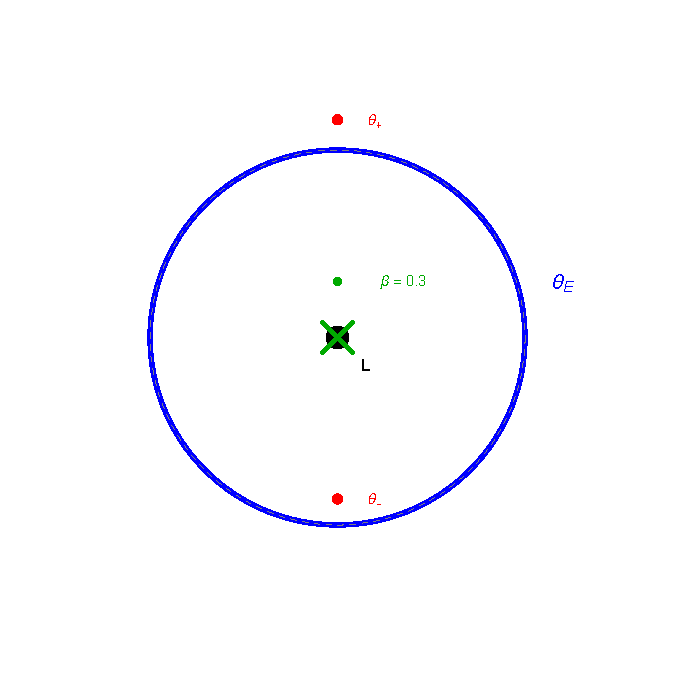
\includegraphics[width=0.65\textwidth]{../Figures/04_Lens_Equation/einstein_ring.pdf}
    \caption{The Einstein ring.  When a source (star symbol at center)
    lies exactly behind a point mass lens (filled circle at center),
    the image is a complete ring of angular radius $\thetaE$.  For a
    slightly offset source ($\beta \neq 0$), the ring breaks into two
    images at positions $\theta_+$ and $\theta_-$.  Generated by
    \texttt{lens\_equation.wl}.}
    \label{fig:einstein_ring}
\end{figure}

\subsection{Numerical Examples}

\begin{example}
\label{ex:einstein_radius_values}
\textbf{Einstein radii for typical lensing systems.}

\medskip
\noindent\textbf{(a) Stellar microlensing} ($M = 1\,\Msun$,
$\Dd \approx \Ds/2 \approx 5$~kpc, $\Dds \approx 5$~kpc):
\begin{equation}
    \thetaE = \sqrt{\frac{4 \times 6.674 \times 10^{-11} \times
    1.989 \times 10^{30}}{(3 \times 10^{8})^2} \times
    \frac{1}{10 \times 3.086 \times 10^{19}}}
    \approx 0.9~\text{mas} \,.
    \label{eq:thetaE_microlensing}
\end{equation}
The Einstein radius for stellar microlensing is of order
\textit{milliarcseconds} --- far too small to resolve the individual
images, but the magnification is detectable photometrically.

\medskip
\noindent\textbf{(b) Galaxy-scale lensing} ($M = 10^{12}\,\Msun$,
$z_d = 0.3$, $z_s = 1$):
With $\Dd \approx 919$~Mpc, $\Ds \approx 1652$~Mpc,
$\Dds \approx 1055$~Mpc:
\begin{equation}
    \thetaE \approx 2.4'' \,.
    \label{eq:thetaE_galaxy}
\end{equation}
Galaxy-scale Einstein radii are of order \textit{arcseconds} ---
easily resolved with ground-based telescopes.  This is the regime
of strong lensing that produces multiple images and arcs.

\medskip
\noindent\textbf{(c) Cluster-scale lensing} ($M_{\mathrm{E}} \sim
2 \times 10^{14}\,\Msun$ inside the Einstein radius,
$z_d = 0.3$, $z_s = 2$):
With $\Dd \approx 919$~Mpc, $\Ds \approx 1727$~Mpc,
$\Dds \approx 1329$~Mpc, the point-mass formula gives:
\begin{equation}
    \thetaE \approx 37'' \,.
    \label{eq:thetaE_cluster}
\end{equation}
Cluster-scale Einstein radii are of order \textit{tens of arcseconds},
producing the spectacular giant arcs observed in massive galaxy
clusters.  Note that for an extended cluster only the mass
\emph{within} the Einstein radius enters the point-mass-equivalent
estimate above; the total virial mass $M_{200} \sim 10^{15}\,\Msun$
of a typical massive cluster is much larger, but most of it lies
outside $\thetaE$.  An NFW treatment (Module~10) yields the same
answer self-consistently.

\medskip
\noindent
These values are computed and verified in
\mathlink{04_Lens_Equation/lens_equation.wl}{lens\_equation.wl}.
Interactive exploration is available in
\mathlink{04_Lens_Equation/einstein_ring.nb}{einstein\_ring.nb}.
\end{example}
\begin{annotation}[Doing the numbers without losing a power of ten]
Two intermediate values are worth memorizing: $4\Gnewton\Msun/\speedoflight^2 = 5.91\times10^{3}$~m
(twice the Sun's Schwarzschild radius), and $1~\mathrm{kpc} = 3.086\times10^{19}$~m.
For case (a), $\Dds/(\Dd\Ds) = 1/(10~\mathrm{kpc})$, so
$\thetaE^2 = 5.91\times10^{3}/3.086\times10^{20} = 1.91\times10^{-17}$ and
$\thetaE = 4.38\times10^{-9}$~rad $= 0.90$~mas. The physical radius is
$\RE = \Dd\thetaE = 6.8\times10^{11}$~m $\approx 4.5$~AU. A useful scaling is
\begin{equation*}
    \thetaE \simeq 0.90~\mathrm{mas}\,
    \Big(\frac{M}{\Msun}\Big)^{1/2}
    \Big(\frac{\Dd\Ds/\Dds}{10~\mathrm{kpc}}\Big)^{-1/2}.
\end{equation*}
Check it on case (b): $\Dd\Ds/\Dds = 1439$~Mpc gives
$0.90~\mathrm{mas}\times10^{6}\times(1.439\times10^{5})^{-1/2} = 2.4''$.
\emph{Classic error:} quoting $\thetaE$ in radians when arcseconds were
meant ($1~\mathrm{rad} = 206265''$).
\end{annotation}


% =====================================================================
\section{Image Positions for a Point Mass Lens}
\label{sec:image_positions}

The two image positions $\theta_\pm$ from eq.~\eqref{eq:image_positions}
have several important properties.  It is convenient to work with the
dimensionless variable $u \equiv \beta / \thetaE$ (source position in
units of the Einstein radius).  Then:
\begin{equation}
    \theta_\pm = \frac{\thetaE}{2}\left(u \pm \sqrt{u^2 + 4}\right) .
    \label{eq:images_dimensionless}
\end{equation}

\subsection{Properties of the Images}

\begin{enumerate}
    \item \textbf{$\theta_+$ is always positive} (on the same side of the
          lens as the source) and satisfies $\theta_+ > \thetaE$.  This
          is the \textbf{primary image}, which is always located
          \textit{outside} the Einstein radius.

    \item \textbf{$\theta_-$ is always negative} (on the opposite side
          of the lens from the source) and satisfies
          $|\theta_-| < \thetaE$.  This is the \textbf{secondary image},
          located \textit{inside} the Einstein radius.  Its negative sign
          indicates opposite parity (the image is mirror-reflected).

    \item \textbf{Sum and product:} From Vieta's formulas applied to
          the quadratic~\eqref{eq:quadratic}:
          \begin{equation}
              \theta_+ + \theta_- = \beta \,, \qquad
              \theta_+\, \theta_- = -\thetaE^2 \,.
              \label{eq:vieta}
          \end{equation}
          The product relation shows that the images always straddle the
          Einstein ring: one inside, one outside.

    \item \textbf{Image separation:}
          \begin{equation}
              \Delta\theta = \theta_+ - \theta_-
              = \sqrt{\beta^2 + 4\,\thetaE^2} \,.
              \label{eq:image_separation}
          \end{equation}
          The minimum separation occurs at $\beta = 0$
          (Einstein ring configuration), where $\Delta\theta = 2\,\thetaE$.
\end{enumerate}
\begin{annotation}[Vieta in practice]
The product relation $\theta_+|\theta_-| = \thetaE^2$ does not depend on
$\beta$. For a point-mass lens, the Einstein radius is the
\emph{geometric mean} of the two image distances from the lens, and it can be read
off without knowing where the source is. The sum relation gives the source
position, $\beta = \theta_+ + \theta_- = \theta_+ - |\theta_-|$.

\emph{A one-line proof of the ordering in item~1--2:} the product is
negative, so the roots have opposite signs. The sum $\beta > 0$ makes the
positive root the larger in magnitude. Two numbers whose product of magnitudes
is $\thetaE^2$ and which are unequal must straddle $\thetaE$:
$\theta_+ > \thetaE > |\theta_-|$.
\end{annotation}

\subsection{Limiting Cases}

\paragraph{Source on the optical axis ($\beta \to 0$, $u \to 0$):}
Both images approach the Einstein radius:
$\theta_+ \to +\thetaE$, $\theta_- \to -\thetaE$.
The two images merge into the \textbf{Einstein ring}.

\paragraph{Source far from the lens ($\beta \gg \thetaE$, $u \gg 1$):}
\begin{align}
    \theta_+ &\approx \beta + \frac{\thetaE^2}{\beta}
    \to \beta \quad \text{(approaches the unlensed position)} \,,
    \label{eq:theta_plus_limit} \\
    \theta_- &\approx -\frac{\thetaE^2}{\beta} \to 0
    \quad \text{(approaches the lens, becomes infinitely demagnified)} \,.
    \label{eq:theta_minus_limit}
\end{align}
In this limit the primary image is essentially at the unlensed source
position (negligible lensing), and the secondary image is extremely
close to the lens and too faint to observe.
\begin{derivation}[The next order in eqs.~\eqref{eq:theta_plus_limit}--\eqref{eq:theta_minus_limit}]
Write $\sqrt{\beta^2 + 4\thetaE^2} = \beta\sqrt{1 + 4\thetaE^2/\beta^2}$ and
expand $\sqrt{1+x} = 1 + x/2 - x^2/8 + \dots$ with $x = 4\thetaE^2/\beta^2$:
$\sqrt{\beta^2 + 4\thetaE^2} = \beta + 2\thetaE^2/\beta - 2\thetaE^4/\beta^3 + \dots$
Halving the sum and difference with $\beta$:
\begin{equation*}
    \theta_+ = \beta + \frac{\thetaE^2}{\beta} - \frac{\thetaE^4}{\beta^3} + \dots,
    \qquad
    \theta_- = -\frac{\thetaE^2}{\beta} + \frac{\thetaE^4}{\beta^3} + \dots
\end{equation*}
The leading correction to $\theta_+$ is the deflection $\alpha(\beta) = \thetaE^2/\beta$
evaluated at the unlensed position, which is what one expects from a single weak kink.
\end{derivation}
\begin{bridge}[Adding a point mass to a smooth lens]
Chapter~\ref{ch:power_law_point_mass} puts a point mass (Einstein radius
$\thetaBH$) at the centre of a power-law galaxy. By superposition
(eq.~\ref{eq:superposition_deflection}) its reduced deflection
$\thetaBH^2/\theta$, derived above, is simply added to the galaxy's.
Because this term diverges as $\theta \to 0$, it dominates exactly where the
galaxy's own central images would form, even when $\thetaBH \ll \thetaE$.
\end{bridge}

\begin{figure}[ht]
    \centering
    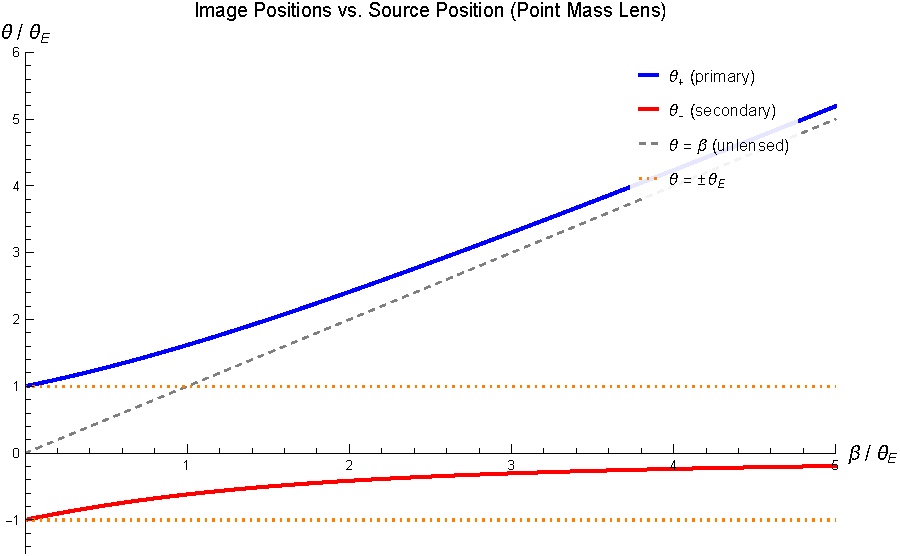
\includegraphics[width=0.78\textwidth]{../Figures/04_Lens_Equation/image_positions.pdf}
    \caption{Image positions $\theta_+$ and $\theta_-$ as functions of
    the source position $\beta$ for a point mass lens, in units of the
    Einstein radius $\thetaE$.  The primary image $\theta_+$ (blue) is
    always outside $\thetaE$ and approaches the unlensed position
    (gray dashed line) for $\beta \gg \thetaE$.  The secondary image
    $\theta_-$ (red) is always inside $\thetaE$ (in absolute value)
    and approaches the lens for $\beta \gg \thetaE$.  At $\beta = 0$,
    both images are at $\pm\thetaE$ (Einstein ring).  Generated by
    \texttt{lens\_equation.wl}.}
    \label{fig:image_positions}
\end{figure}


% =====================================================================
\section{Magnification of a Point Mass Lens}
\label{sec:magnification_preview}

Gravitational lensing conserves surface brightness (a consequence of
Liouville's theorem applied to the photon phase space), but it changes
the \textit{solid angle} subtended by the image compared to the source.
The ratio of image area to source area is the \textbf{magnification}
$\mu$.  We will derive the magnification formalism rigorously in
Module~5; here we preview the key results for the point mass lens.

For a circularly symmetric lens, the magnification is
(Narayan \& Bartelmann eq.~26):
\begin{equation}
    \mu = \frac{\theta}{\beta}\, \frac{d\theta}{d\beta} \,.
    \label{eq:magnification_circular}
\end{equation}
The first factor accounts for the tangential stretching of the image
(the image is at a different angular radius than the source), and
the second factor accounts for the radial stretching.
\begin{derivation}[Where $\mu = (\theta/\beta)(d\theta/d\beta)$ comes from]
Surface brightness is conserved, so flux ratio $=$ solid-angle ratio. In polar
coordinates centred on the lens, an image element has area
$\theta\,d\theta\,d\phi$ and the corresponding source element
$\beta\,d\beta\,d\phi$. The polar angle $d\phi$ is the \emph{same} in both
because an axisymmetric deflection is purely radial. Therefore
\begin{equation*}
    \mu = \frac{\theta\,d\theta\,d\phi}{\beta\,d\beta\,d\phi}
        = \underbrace{\frac{\theta}{\beta}}_{\text{tangential}}\;
          \underbrace{\frac{d\theta}{d\beta}}_{\text{radial}},
    \qquad
    \mu^{-1} = \frac{\beta}{\theta}\,\frac{d\beta}{d\theta}
    = \Big(1 - \frac{\alpha}{\theta}\Big)\Big(1 - \frac{d\alpha}{d\theta}\Big)
\end{equation*}
(Congdon \& Keeton eq.~2.23). This is the determinant of the map
$(\theta\cos\phi, \theta\sin\phi) \mapsto (\beta\cos\phi, \beta\sin\phi)$.
Module~\ref{ch:magnification} shows that the two factors are the eigenvalues
$\lambda_t = 1 - \alpha/\theta$ and $\lambda_r = 1 - d\alpha/d\theta$ of the
Jacobian. For the point mass $\lambda_t = 1 - \thetaE^2/\theta^2$ and
$\lambda_r = 1 + \thetaE^2/\theta^2$, whose product is the denominator
$1 - \thetaE^4/\theta^4$ of eq.~\eqref{eq:magnification_pm}.
\end{derivation}

For the point mass lens equation $\beta = \theta - \thetaE^2/\theta$,
we have $d\beta/d\theta = 1 + \thetaE^2/\theta^2$, and the
magnification of each image is:
\begin{equation}
    \mu_\pm = \frac{\theta_\pm}{\beta}\,
    \frac{1}{1 + \thetaE^2/\theta_\pm^2}
    = \frac{\theta_\pm^4}{\theta_\pm^4 - \thetaE^4} \,.
    \label{eq:magnification_pm}
\end{equation}

Using the dimensionless variable $u = \beta/\thetaE$, the magnifications
simplify to (Narayan \& Bartelmann eq.~27):
\begin{equation}
    \boxed{
    \mu_\pm = \frac{u^2 + 2}{2u\sqrt{u^2 + 4}} \pm \frac{1}{2}
    }
    \label{eq:magnification_u}
\end{equation}
\begin{derivation}[From eq.~\eqref{eq:magnification_pm} to eq.~\eqref{eq:magnification_u}]
Let $x_\pm = \theta_\pm/\thetaE = (u \pm \sqrt{u^2+4})/2$, so
$\mu(x) = x^4/(x^4 - 1)$.
\begin{enumerate}
    \item Vieta for $x^2 - ux - 1 = 0$: $x_+x_- = -1$, so $x_- = -1/x_+$ and
          $x_-^4 = 1/x_+^4$.
    \item Hence $\mu_- = \frac{x_+^{-4}}{x_+^{-4} - 1} = \frac{1}{1 - x_+^4}$
          and the \emph{signed} magnifications add to one:
          $\mu_+ + \mu_- = \frac{x_+^4 - 1}{x_+^4 - 1} = 1$.
    \item Their difference is
          $\mu_+ - \mu_- = \frac{x_+^4 + 1}{x_+^4 - 1}
          = \frac{x_+^2 + x_-^2}{x_+^2 - x_-^2}$
          (divide top and bottom by $x_+^2$, use $x_+^{-2} = x_-^2$).
    \item From the sum $x_+ + x_- = u$ and the difference
          $x_+ - x_- = \sqrt{u^2+4}$:
          $x_+^2 + x_-^2 = (x_+ + x_-)^2 - 2x_+x_- = u^2 + 2$ and
          $x_+^2 - x_-^2 = (x_+ + x_-)(x_+ - x_-) = u\sqrt{u^2+4}$.
    \item So $\mu_\pm = \tfrac12[(\mu_+ + \mu_-) \pm (\mu_+ - \mu_-)]
          = \tfrac12 \pm \frac{u^2+2}{2u\sqrt{u^2+4}}$ (signed), i.e.\
          $|\mu_\pm| = \frac{u^2+2}{2u\sqrt{u^2+4}} \pm \tfrac12$.
\end{enumerate}
\end{derivation}

Several important properties follow:
\begin{itemize}
    \item $\mu_+ > 0$ always (same parity as the source).
    \item $\mu_- < 0$ always (opposite parity --- the image is
          mirror-reflected), because $|\theta_-| < \thetaE$ makes the
          denominator of eq.~\eqref{eq:magnification_pm} negative.  As in
          Narayan \& Bartelmann eq.~27, the lower sign in
          eq.~\eqref{eq:magnification_u} gives the \textit{absolute}
          magnification $|\mu_-|$; the signed value is
          $\mu_- = \frac{1}{2} - \frac{u^2+2}{2u\sqrt{u^2+4}}$.
    \item The total magnification (sum of absolute values) is:
          \begin{equation}
              |\mu_+| + |\mu_-| = \frac{u^2 + 2}{u\sqrt{u^2 + 4}} > 1
              \quad \text{for all } u > 0 \,.
              \label{eq:total_magnification}
          \end{equation}
          Gravitational lensing always \textit{increases} the total
          observed flux (the total magnification exceeds unity).
    \item As $u \to 0$ (source on the optical axis), both
          $|\mu_\pm| \to \infty$: the Einstein ring is
          \textit{infinitely} magnified (in the geometric optics
          approximation).
    \item As $u \to \infty$, $\mu_+ \to 1$ (unlensed) and
          $|\mu_-| \to 0$ (secondary image disappears).
\end{itemize}
\begin{annotation}[Signed vs.\ absolute magnification]
The sign of $\mu$ is the \emph{parity}. A negative $\mu$ means that the image is a
mirror image of the source (Module~\ref{ch:magnification}: $\mu = 1/\det\Amat$).
Fluxes add as $|\mu|$, so the total brightening is $|\mu_+| + |\mu_-|$, whereas
the signed sum is identically $\mu_+ + \mu_- = 1$ (previous derivation).
Equivalently, $|\mu_+| - |\mu_-| = 1$ exactly.
\emph{Numbers to remember:} at $u = 1$ (source on the Einstein circle)
$|\mu_+| = 1.171$, $|\mu_-| = 0.171$, total $1.342$ (Narayan \& Bartelmann
eq.~29). This is the classic microlensing detection threshold. As $u \to 0$ the
total grows as $1/u$, the point-source divergence that a finite source
regularizes.

\emph{Classic error:} adding signed magnifications to get the total flux.
That always gives exactly 1, which is a good check of your signs but not a flux.
\end{annotation}
\begin{bridge}[Parity, and a lens with an even number of images]
The point mass produces \emph{two} images, one of each parity. A smooth,
non-singular lens always produces an \emph{odd} number (for a source not on
a caustic). The point mass
escapes that theorem because its density is singular: the would-be third
image is swallowed at $\theta = 0$. Chapter~\ref{ch:odd_images} uses exactly
this mechanism. A central point mass in a galaxy punctures the smooth
$\Sigma$ that the odd-number theorem assumes, and can suppress the faint
central image.
\end{bridge}


% =====================================================================
\section{Summary}
\label{sec:lens_eq_summary}

\begin{itemize}
    \item The \textbf{thin-screen approximation} projects the
          three-dimensional mass distribution onto a single lens plane,
          justified by the small ratio of lens extent to cosmological
          distance ($\sim 10^{-4}$).

    \item The \textbf{lens equation}
          $\vecbeta = \vectheta - \vecalpha(\vectheta)$ maps image
          positions to source positions.  The \textbf{reduced deflection
          angle} $\vecalpha = (\Dds/\Ds)\,\boldsymbol{\hat{\alpha}}$
          absorbs the distance factors.

    \item The \textbf{surface mass density} $\Sigma(\vecxi)$ and
          the deflection integral~\eqref{eq:deflection_integral_continuous} allow
          the treatment of arbitrary continuous mass distributions.

    \item The \textbf{critical surface mass density}
          $\Sigmacr = (\speedoflight^2 / 4\pi\Gnewton)\, (\Ds / \Dd\,\Dds)$
          separates weak lensing ($\kappab < 1$) from strong lensing
          ($\kappab \geq 1$).

    \item The \textbf{Einstein radius}
          $\thetaE = \sqrt{4\Gnewton M / \speedoflight^2 \cdot
          \Dds / (\Dd\,\Ds)}$ is the characteristic angular scale of
          lensing.  Typical values: $\sim 1$~mas for stellar microlensing,
          $\sim 1''$--$3''$ for galaxy lensing ($M \sim 10^{11}$--$10^{12}\,\Msun$),
          $\sim 30''$--$40''$ for cluster lensing.

    \item A \textbf{point mass lens} always produces two images:
          $\theta_\pm = (\beta \pm \sqrt{\beta^2 + 4\thetaE^2})/2$.
          The primary image ($\theta_+$) is outside $\thetaE$ with the
          same parity; the secondary ($\theta_-$) is inside $\thetaE$
          with opposite parity.

    \item When the source is exactly behind the lens ($\beta = 0$), the
          images merge into an \textbf{Einstein ring} at angular radius
          $\thetaE$.

    \item The \textbf{magnification} of the point mass lens is
          $\mu_\pm = (u^2 + 2) / (2u\sqrt{u^2 + 4}) \pm 1/2$, where
          $u = \beta/\thetaE$.  The total magnification always exceeds
          unity.
\end{itemize}


% =====================================================================
\section{Problems}
\label{sec:lens_eq_problems}

\begin{exercise}
\label{ex:derive_lens_eq}
\textbf{(Derivation of the lens equation.)}
Starting from the lensing geometry (Figure~\ref{fig:lensing_geometry}),
derive the lens equation~\eqref{eq:lens_equation_full}.
\begin{enumerate}[label=(\alph*)]
    \item Using the small-angle approximation, show that the physical
          position in the source plane is
          $\veceta = (\Ds/\Dd)\,\vecxi - \Dds\,\boldsymbol{\hat{\alpha}}(\vecxi)$.
    \item Substitute $\vecxi = \Dd\,\vectheta$ and
          $\veceta = \Ds\,\vecbeta$ to obtain the lens equation in
          angular coordinates.
    \item Define the reduced deflection angle and write the lens equation
          in the compact form $\vecbeta = \vectheta - \vecalpha(\vectheta)$.
\end{enumerate}
\end{exercise}

\begin{exercise}
\label{ex:point_mass_solve}
\textbf{(Point mass lens equation.)}
For a point mass lens with Einstein radius $\thetaE$:
\begin{enumerate}[label=(\alph*)]
    \item Derive the lens equation $\beta = \theta - \thetaE^2/\theta$
          from the deflection angle $\alphahat = 4\Gnewton M /
          (\speedoflight^2 \xi)$.
    \item Solve the resulting quadratic to obtain the image positions
          $\theta_\pm$.
    \item Show that two images always form (i.e., the discriminant is
          always positive).
    \item Verify the Vieta relations: $\theta_+ + \theta_- = \beta$
          and $\theta_+\,\theta_- = -\thetaE^2$.
    \item Show that $\theta_+ > \thetaE > 0 > \theta_- > -\thetaE$
          for $\beta > 0$.
\end{enumerate}
Verify with
\solnlink{04_Lens_Equation/problems\_04.wl}{problems\_04.wl}.
\end{exercise}

\begin{exercise}
\label{ex:einstein_radius_compute}
\textbf{(Einstein radius for various systems.)}
Compute the Einstein radius $\thetaE$ for:
\begin{enumerate}[label=(\alph*)]
    \item \textbf{Stellar microlensing:} $M = 1\,\Msun$, lens at
          distance $\Dd = 5$~kpc, source at $\Ds = 10$~kpc (so
          $\Dds = 5$~kpc).  Express the result in milliarcseconds.
    \item \textbf{Galaxy lensing:} $M = 10^{12}\,\Msun$, $z_d = 0.3$,
          $z_s = 1$.  Use the angular diameter distances from
          Module~3 (or the Mathematica script):
          $\Dd \approx 919$~Mpc, $\Ds \approx 1652$~Mpc,
          $\Dds \approx 1055$~Mpc.  Express the result in arcseconds.
    \item \textbf{Cluster lensing:} $M = 10^{15}\,\Msun$, $z_d = 0.3$,
          $z_s = 2$.  Use $\Dd \approx 919$~Mpc, $\Ds \approx 1727$~Mpc,
          $\Dds \approx 1329$~Mpc.  Express the result in arcseconds.
\end{enumerate}
For each case, also compute the physical Einstein radius $\RE = \Dd\,\thetaE$
in kpc.  Verify with
\solnlink{04_Lens_Equation/problems\_04.wl}{problems\_04.wl}.
\end{exercise}

\begin{exercise}
\label{ex:sigma_cr_compute}
\textbf{(Critical surface mass density.)}
\begin{enumerate}[label=(\alph*)]
    \item Starting from the definition~\eqref{eq:sigma_cr}, verify that
          $\Sigmacr$ has units of mass per area by performing a
          dimensional analysis.
    \item Compute $\Sigmacr$ (in g\,cm$^{-2}$ and $\Msun$\,pc$^{-2}$)
          for the galaxy lens configuration of
          Exercise~\ref{ex:einstein_radius_compute}(b).
    \item Compute $\Sigmacr$ for the cluster lens configuration of
          Exercise~\ref{ex:einstein_radius_compute}(c).
    \item A typical elliptical galaxy has a central surface mass density
          of $\Sigma_0 \approx 5000\,\Msun$\,pc$^{-2}$.  Is it a
          strong lens?  Compare $\Sigma_0$ with your result from~(b).
\end{enumerate}
Verify with
\solnlink{04_Lens_Equation/problems\_04.wl}{problems\_04.wl}.
\end{exercise}

\begin{exercise}
\label{ex:image_positions_plot}
\textbf{(Image positions for a point mass lens.)}
Consider a point mass lens with $\thetaE = 1''$.
\begin{enumerate}[label=(\alph*)]
    \item For source positions $\beta = 0.1'', 0.5'', 1'', 2'', 5''$,
          compute both image positions $\theta_+$ and $\theta_-$.
          Tabulate your results.
    \item Plot $\theta_+$ and $\theta_-$ as functions of $\beta$ for
          $0 \leq \beta \leq 5''$.  On your plot, also show the
          Einstein radius and the line $\theta = \beta$ (unlensed
          position).
    \item Compute the image separation $\Delta\theta = \theta_+ - \theta_-$
          for each value of $\beta$ and plot it.  What is the minimum
          image separation?
    \item Compute the magnification of each image using
          eq.~\eqref{eq:magnification_u} and plot the total
          magnification $|\mu_+| + |\mu_-|$ as a function of $\beta$.
\end{enumerate}
Use Mathematica to generate the plots and verify the numerical values.
See \mathlink{04_Lens_Equation/lens_equation.wl}{lens\_equation.wl}
and \solnlink{04_Lens_Equation/problems\_04.wl}{problems\_04.wl}.
\end{exercise}
